% 阶段报告五：中文正式版。编译：xelatex stage_report_5_zh.tex（两遍）。
% 数字来源及独立核验见本目录 verified_numbers.json 和 README.md。
\documentclass[11pt,a4paper,UTF8,fontset=fandol]{ctexart}
\usepackage[margin=0.9in]{geometry}
\usepackage{amsmath,amssymb,booktabs,tabularx,array,graphicx,xcolor,float}
\usepackage[hidelinks]{hyperref}
\usepackage{enumitem}
\setlist{itemsep=3pt,topsep=5pt}
\renewcommand{\refname}{参考文献}
\newcolumntype{Y}{>{\raggedright\arraybackslash}X}
\newcommand{\code}[1]{\nolinkurl{#1}}
\emergencystretch=3em
\linespread{1.15}
\setlength{\parindent}{2em}
\setlength{\parskip}{0pt}
% 页眉沿用 ctexart 默认 headings 样式，但保留节标题原大小写（E1-T 不被改写）。
\makeatletter
\renewcommand\sectionmark[1]{\markboth{\ifnum\c@secnumdepth>\z@\thesection\quad\fi #1}{}}
\makeatother
\title{\bfseries 分型缺口能否补上，候选标签是否可信：上限诊断、共识审计与效用学习\\[7pt]
\large PanNuke 细胞核实例分割：阶段报告五}
\author{课程项目 bdd26}
\date{2026 年 10 月 13 日\\\small 实验范围：2026 年 10 月 9 日至 12 日}
\begin{document}
\maketitle

\begin{abstract}
阶段报告四结束后，项目留下两个悬而未决的问题：已检出细胞核的分类误差还能通过学习减少多少；两倍尺度补入的候选中，未匹配到标注的那部分究竟是什么，标签本身是否可靠。本阶段用五项实验回答这两个问题。分类上限诊断显示，保持实例轮廓不变、仅把已匹配对象改成真值类别，三划分平均 mPQ 从 0.4995 升至 0.6632；其中真值属于 Inflammatory/Connective 的修正贡献约七成。随后的预注册探针 T0--T3 检验简单分类器能否实现这部分改善：最优配置仅 $+0.0002$（置信区间跨零），未加权线性头的 Dead PQ 下降 $0.0053$ 超出预设的容许幅度，未达到通过条件，冻结特征的事后重分型路线就此结束。独立盲审因缺少人类专家评审资源而转为无专家方案：13 席跨折检测器对冻结候选的支持度远超合成空对照（支持度 $\geq$3 的比例 0.75\% 对 66--73\%），真值匹配率随支持度单调上升；两轮模型预审彼此一致性差（kappa $-0.09$ 至 $+0.35$），不可用。在此基础上，E1-T 分型共识审计显示，基模型分错的已匹配实例上，12 席评审团的多数类与基类一致的比例为 72.5\% [0.706, 0.742]，与真值类一致仅 18.2\%，两个置信区间不重叠，而基模型分对实例上的改判率只有 1.9\%——按预注册判读规则，Inflammatory/Connective 标签边界模糊的检测器一致性证据成立。E3 候选质量学习把上述支持度纳入特征：候选匹配概率可预测（交叉验证 AUC 0.721/0.737），但沿用冻结选择规则时，此次新增的全部候选配置均未达到 strict Dead 下限，主要判定条件与次要判定条件在三组方案上均未通过，按预注册规则停止该方向的实验。T、E1-C、E1-M、E1-T、E3 均未读取测试折；上限诊断使用了历史测试预测。本阶段仅拟合线性分类器和逻辑回归，未新增分割模型训练；此前全量测试 335 项通过，终版产物经评审后重新生成；除 E3 的 bootstrap mPQ 统计口径修正外，与首版逐位一致。
\end{abstract}
\noindent\textbf{关键词：}细胞核实例分割；PanNuke；标签噪声；检测器共识；预注册检验；候选筛选

\section{研究背景与本阶段问题}

阶段报告四厘清了两倍尺度的机制与成本\cite{reports}：HV 面积门槛只解释小部分尺度增益，Dead 专家分支因梯度冲突前提不成立而按预注册规则停止，两模型系统约需单模型 6.1 倍推理时间。EF-P2 保留为机制证据和教师候选。在此之后，研究的重心从“再找一个检测改进”转向两个更基础的问题。

第一是\textbf{分型缺口}。基线 CellViT-UNI 的官方三划分 mPQ 为 0.4995，不区分类别的 bPQ 为 0.6653。两者之差意味着相当一部分已检出的核被分错了类别。此前 CONCH 实例重分类的负结果\cite{structure}说明所测试的外部图文特征未带来改善，但当前模型自身特征里还有没有可利用的分型信息，尚未直接检验。

第二是\textbf{候选与标签}。EF-P2 从两倍尺度模型补入的候选中，53--61\% 没有匹配到任何真值实例（验证折 55.8\%，测试折历史口径 57--61\%）。它们可能是碎屑、轮廓偏差，也可能是真实存在但被标注遗漏的核。10 月 9 日的建议稿\cite{next}据此提出了两项并行实验：固定几何的分型初筛（T 实验）与独立候选盲审（E1）。

本阶段根据实验结果和评审资源调整了后续安排。T 实验未通过预注册条件后，E1 又因缺少人类专家评审资源而改为无专家方案，随后派生出两项新实验（E1-T 分型共识、E3 候选质量学习），二者均在启动前预注册\cite{specs}。全文按时间顺序报告这五项工作：第 2 节分类上限诊断，第 3 节 T0--T3，第 4 节 E1 材料包与无专家修订（E1-C/E1-M），第 5 节 E1-T，第 6 节 E3，第 7 节复核记录。

数据边界的约定与前一阶段相同。T、E1-C、E1-M、E1-T、E3 五项实验只使用训练折与验证折，未读取任何测试折；除 E1-C 为评审团补入的两席 HoVer-Net 验证折推理外，没有新的 GPU 推理，也未新增分割模型训练。第 2 节的上限诊断是唯一的例外：它读取了已冻结、已经评测过的三划分测试预测，属于审计型访问，只读不调参，下文单独说明。

\section{分类上限诊断：理想改类能到多少}

这个诊断回答一个朴素的问题：如果每个已检出的核都被赋予正确类别，指标能到多少？做法是读取冻结的基线测试预测（无 TTA、最终检查点），保持实例数量与轮廓完全不变，只把 IoU$>0.5$ 的已匹配对象改成其真值类别，再用与官方评测一致的评测器重算 mPQ\cite{structure}。这类使用真值的理想化干预称为 oracle，它给出的是“保持现有轮廓、纠正已匹配实例类别后的指标”，不是模型可达成绩。

\begin{table}[H]
\centering\small
\caption{分类上限诊断（三划分平均，实例几何不变，仅改已匹配对象的类别）。第三行只修正真值属于 Inflammatory 或 Connective 的已匹配对象，不论其原预测为何。}
\label{tab:oracle}
\begin{tabular}{lrr}\toprule
干预 & 三划分平均 mPQ & 相对原始\\\midrule
原始类别 & 0.49951 & —\\
全部已匹配对象按真值改类别 & 0.66322 & $+0.16371$\\
真值为 Inf/Conn 的已匹配对象按真值改类别 & 0.61412 & $+0.11461$\\
\bottomrule
\end{tabular}
\end{table}

三划分逐项为 $+0.169/+0.167/+0.155$，方向一致。split 1 的逐类变化（原始$\to$全类别 oracle）为：Neoplastic $0.570\to0.666$，Inflammatory $0.440\to0.720$，Connective $0.418\to0.595$，Dead $0.142\to0.411$，Epithelial $0.575\to0.659$。Inflammatory 与 Connective 的抬升幅度最大；Dead 的绝对空间也很大，但它同时受漏检约束（漏检的核没有改类的机会）。

第三行约占第二行增益的 70\%。这个比例需要小心表述：脚本只按\textbf{真值类别}筛选修正对象，包含了这两类被错分成任何类别的情况，修正也会减少其他类别的误报计数；mPQ 是非线性指标，70\% 不是可相加的类别贡献分解\cite{structure}。同样，oracle mPQ 0.6632 与 bPQ 0.6653 数值接近只是巧合，两者的匹配与汇总口径不同。

这次诊断访问了历史测试产物且未预注册，只能用于提出假设。它提出的假设很直接：分型缺口值得检验，而 Inf/Conn 边界是优先检查的类别组合。随后三节的实验都在验证折上检验这条线。

\section{T0--T3：固定几何的分型探针}

\subsection{设计与通过条件}

T 实验\cite{specs}的假设是：不改动核的数量和轮廓时，实例级特征里可能仍有像素多数票没有用上的类别信息。开发限定 split 1：fold 1（63,218 个真值实例）训练读出头，fold 2（59,593 个预测实例）验证，fold 3 不读。四个配置在启动前冻结：

\begin{table}[H]
\centering\small
\caption{T0--T3 配置与验证折结果（mPQ，相对 T0 之差）。T1 的方括号为配对图像 bootstrap 95\% 区间。}
\label{tab:t}
\begin{tabular}{llrr}\toprule
配置 & 内容 & mPQ & $\Delta$ vs T0\\\midrule
T0 & 像素多数票（现行解码） & 0.483486 & —\\
T1 & 实例内类别概率均值 & 0.483182 & $-0.0003$ [$-0.0010,+0.0003$]\\
T2 & 冻结 TP 特征实例池化 + 线性头 & 0.483707 & $+0.0002$ [$-0.0027,+0.0019$]\\
T3 & T2 + 24px 上下文环（等维求和） & 0.481796 & $-0.0017$\\
\bottomrule
\end{tabular}
\end{table}

T0 精确复现官方 fold 2 评测；T2 报两个线性头种子（0.483606/0.483807）的均值，两种子同向。通过条件共六条，要求同时满足：$\Delta\text{mPQ}\geq+0.003$、区间下界大于零、strict mPQ 不降、Dead PQ 下降不超过 $0.002$、超过 T1、种子方向一致。

\subsection{结果：未达到通过条件}

六条中只有三条通过。$+0.0002$ 远低于 $0.003$ 的最低增量，区间下界 $-0.0027$ 小于零；更关键的是第四项限制：未加权线性头的 Dead PQ 相对 T0 下降 $0.0053$，超出 $0.002$ 的容许幅度——简单分类器未改善总体指标，还降低了最稀有类别的表现。使用 sklearn 的确定性实现复核方向一致（0.4817，更差）。按预注册规则：不加大分类器，不加配置，先定位失败原因。

失败位置可以从三个准确率看出来。线性头在\textbf{真值区域}上的诊断准确率为 85.3\%；它在验证折\textbf{匹配预测实例}上的分型准确率为 85.8\%；而现行多数票在同一批实例上是 85.6\%。三个数字几乎相同：线性头从冻结特征里读出的，正是 TP 分支已经在用的信息，未提供额外的有效分类信息；GT 特征导出耗时 790 ms/图（未优化单线程），该诊断耗时不能作为部署效率的依据。T1 的 $-0.0003$ 同时说明此次调整聚合规则未带来改善。

与 CONCH 负结果合并，结论是：两个彼此独立的特征来源（外部病理 VLM、模型内部冻结特征）在本项目已测试的事后分类方案中均未改善分型。bPQ 与 mPQ 之间的分型缺口，未能通过此次更换分类头得到改善。这为两种解释留下空间——标签本身模糊，或收益必须来自联合训练——前者由第 5 节的 E1-T 检验，后者暂不开展实验。

\section{E1 的转折：从人类盲审到检测器共识}

\subsection{材料包与原协议}

E1 原计划由两名合格评审对候选做两阶段盲审。材料包已按预注册生成\cite{specs}：200 个窗口，四类来源各 50 个——x1 已检出的对象（S1）、EF-P2 接受的补入候选（S2）、被拒绝的候选（S3）、随机背景（S4），按组织与触边状态分层抽样并记录入样概率；第一阶段只给图像与十字标记，第二阶段才展示候选与真值轮廓；分析脚本在任何人给出答案之前提交入库。2026 年 10 月 11 日，用户确认人类专家评审在可预见的未来无法获得资源。E1 的人类评审路径就此\textbf{因资源不足而未执行}：材料包保持不变，尚未完成的专家评审要求仍有记录，未来若能安排专家评审仍可执行原协议。

经用户批准，E1 转入无专家方案（spec \S7 修订）：通过跨折检测器共识（E1-C）提供间接证据，以非专家模型预审（E1-M）检验“模型评审”这条低成本路径是否可用。E1-C 提供\textbf{检测器一致性证据}，E1-M 仅验证模型评审流程；两者均不作生物学判断。

\subsection{E1-C：候选的跨检测器共识}

评审团 13 席：split 1 与 split 3 的三种子 $\times$ \{x1, x2\} 共 11 席 CellViT，加 HoVer-Net 两席（split 1 与 split 3 各一席，fold 2 推理，验证折管线检查的 mPQ 0.4509/0.4437）。全部成员的训练折属于 \{1, 3\}，fold 2 从未参与任何成员的训练。候选为 split1\_seed1 的冻结合格池 4,084 个（接受 1,515、拒绝 2,569），支持度定义为与候选 IoU$\geq$0.3 的成员数。

共识证据需要一个对照来定标。合成空对照\cite{specs}在真值实例膨胀 8 像素之外随机放置同面积圆盘（面积重采样自零重叠候选分布，$n=2{,}000$）：平均支持度 0.07，$\geq$3 的比例 0.75\%，$\leq$1 的比例 99.1\%。也就是说，随机位置很少获得多个检测器的共同支持。这个对照控制的只是随机基线，不控制检测器家族共享的核状误报模式。

\begin{table}[H]
\centering\small
\caption{E1-C 按支持度的真值匹配率（IoU$>$0.5）。支持度为 13 席中与候选 IoU$\geq$0.3 的成员数。}
\label{tab:e1c}
\begin{tabular}{lrrrr}\toprule
候选组 & 数量 & 平均支持度 & 支持 0--2 匹配率 & 支持 $\geq$5 匹配率\\\midrule
S2（EF-P2 接受） & 1,515 & 5.47 & 9.6\% & 55.3\%\\
S3（EF-P2 拒绝） & 2,569 & 5.04 & 8.5\% & 45.0\%\\
合成空对照 & 2,000 & 0.07 & \multicolumn{2}{c}{$\geq$3 比例 0.75\%}\\
\bottomrule
\end{tabular}
\end{table}

\begin{figure}[H]
\centering
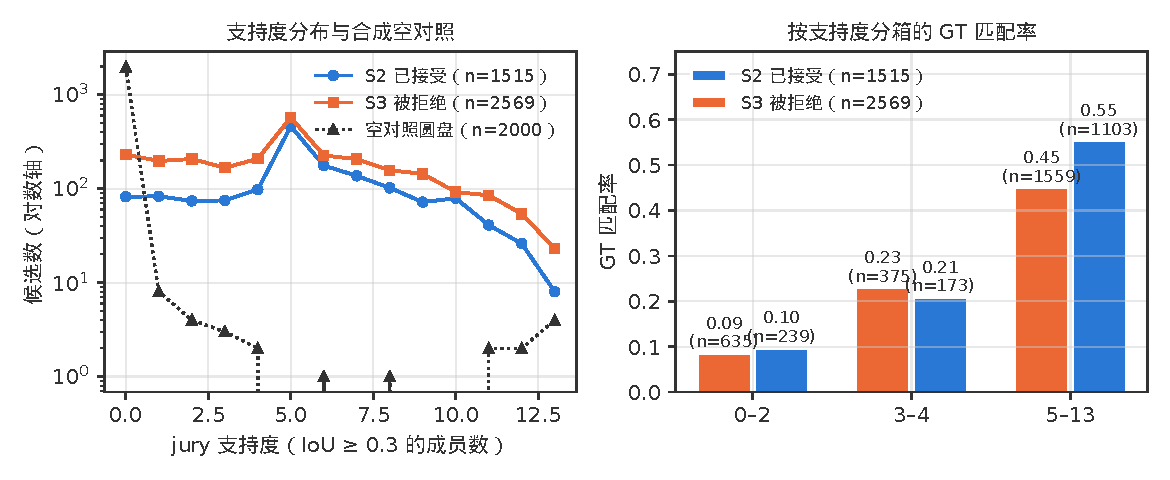
\includegraphics[width=\linewidth]{figs/e1c_support_zh.pdf}
\caption{E1-C 支持度分布与按支持度分箱的真值匹配率。左：候选的支持度集中在 5--7 席，合成空对照几乎全在 0--1 席（对数轴）。右：真值匹配率随支持度单调上升。}
\label{fig:e1c}
\end{figure}

两个来源的候选（无论 EF 规则接受与否）支持度都集中在 5--7 席，与空对照相比，获得多票支持的比例高约两个数量级；真值匹配率随支持度单调上升。按与真值的关系分层后，可进一步区分几种情况：

\begin{itemize}
\item \textbf{与真值零重叠}的候选（S2 518 个、S3 1,146 个）平均支持度 4.8/4.4，其中获得 $\geq$3 席\textbf{且跨训练折、跨架构}支持的分别有 380 个（73.4\%）与 751 个（65.5\%）。这些检测器使用其他折的标注核进行训练；它们在真值未覆盖的位置一致检出了核状对象，构成\textbf{标签可疑的检测器一致性证据}。可能的解释包括标注单位差异、退化或凋亡对象被跳过、检测器家族共享误报模式，本实验不区分。
\item \textbf{有重叠但未达匹配线}（$0<\text{IoU}\leq0.5$）的候选（S2 328 个、S3 582 个）支持度同样高。这与轮廓或实例单位不一致的机制相容：对象被看见了，但边界画法与标注不同。
\item \textbf{可能包含碎屑}（支持 $\leq$1）的未匹配候选占 S2 的 10.0\%、S3 的 15.5\%。EF 的面积过滤与该子群方向一致，但区分能力有限。
\end{itemize}

据此，10 月 11 日的后续计划将支持度纳入候选质量预测：它与匹配率呈单调关系，两个候选来源方向一致，并有随机空对照作为参照，“低维特征 + 评审团支持度”的候选质量学习获得了证据基础。这就是第 6 节 E3 的由来。限制也如实记录：单一 (split1\_seed1) 候选池；CellViT 占 11/13 席，跨架构证据主要靠两席 HoVer-Net；空对照是合成圆盘，不是核状形状。

\subsection{E1-M：模型预审不可用}

材料包的 200 个窗口还用于检验“用视觉模型当评审”是否可行。两轮独立盲评分别使用图像分析通道（passA）与另一模型的原生视觉通道（passB），标注者均为非专家模型。结果：passA 对 S1——几乎全为真实核的 x1 检出对象——只判 40.9\% 为真，存在系统性“非核”偏置，理由高度模板化；passB 排序大体合理（S1 91.5\% $>$ S2 50.6\%/S3 57.3\% $>$ S4 40.8\%）但不确定率高达 34--70\%。两轮之间原始一致率 0.18--0.38，kappa $-0.09$ 至 $+0.35$：\textbf{两轮模型评审的一致性不足}。E1-M 仅完成其流程验证目的，其结果支持预注册方案中不将模型评审纳入正式结论的安排。

\section{E1-T：分型共识与标签边界}

\subsection{设计与预注册判读规则}

T 实验失败后留下的第一个待检验解释是“Inf/Conn 标签模糊”。E1-T\cite{specs}沿用 E1-C 的间接验证思路检验这一解释：在基模型（split1\_seed1，x1，identity 解码）\textbf{分错类别}的已匹配实例上，未参与该预测的检测器是否系统性地支持基模型的类别而非真值类别？

评审团为 E1-C 的 13 席去掉基模型本身，剩 12 席（CellViT 10 + HoVer-Net 2，训练折 \{1, 3\}）。全部计算是缓存重放，CPU 完成，只读 fold 2。实例配对与官方评测一致（IoU$>0.5$，并列时单列）；成员对某真值实例的类型票取其最大 IoU 实例（IoU$\geq0.3$ 才计票）的像素多数票类别。多数类的定义与基模型和真值都无关：总票 $\geq3$、严格胜出、且最高类收到两个训练折的票，否则记“无多数”。分组：G1 = 基分错（6,858 个），G0 = 基分对（40,558 个）；另有未匹配真值 12,456 个与歧义 0 个，合计 59,872，与 fold 2 真值实例总数核对一致。

预注册判读规则写明：若 G1 的 Inf/Conn 混淆组中“多数类 $=$ 基类”的比例高于“多数类 $=$ 真值类”，且聚类 bootstrap 区间分离，并高于 G0 的改判率，则“Inf/Conn 标签边界模糊（检测器一致性证据）”成立；否则将结果归因于模型局限，并结束该方向。Dead 的模式无论方向都单列，不并入结论。

\subsection{结果：多数票更常与基模型类别一致}

\begin{table}[H]
\centering\small
\caption{E1-T 主结果。方括号为图像聚类 bootstrap 95\% 区间（2,000 次，种子 20261011）。}
\label{tab:e1t}
\begin{tabular}{lrr}\toprule
统计量 & 比例 & 95\% 区间\\\midrule
G1：多数类 $=$ 基类 & \textbf{72.5\%}（4,970/6,858） & [0.706, 0.742]\\
G1：多数类 $=$ 真值类 & 18.2\%（1,246/6,858） & [0.167, 0.197]\\
G1：多数类为其他类 & 3.6\%（247） & —\\
G1：无多数 & 5.8\%（395） & [0.052, 0.064]\\
G0：多数类 $\neq$ 真值类（正确分类实例的改判率） & \textbf{1.9\%}（767/40,558） & [0.017, 0.021]\\
\bottomrule
\end{tabular}
\end{table}

\begin{figure}[H]
\centering
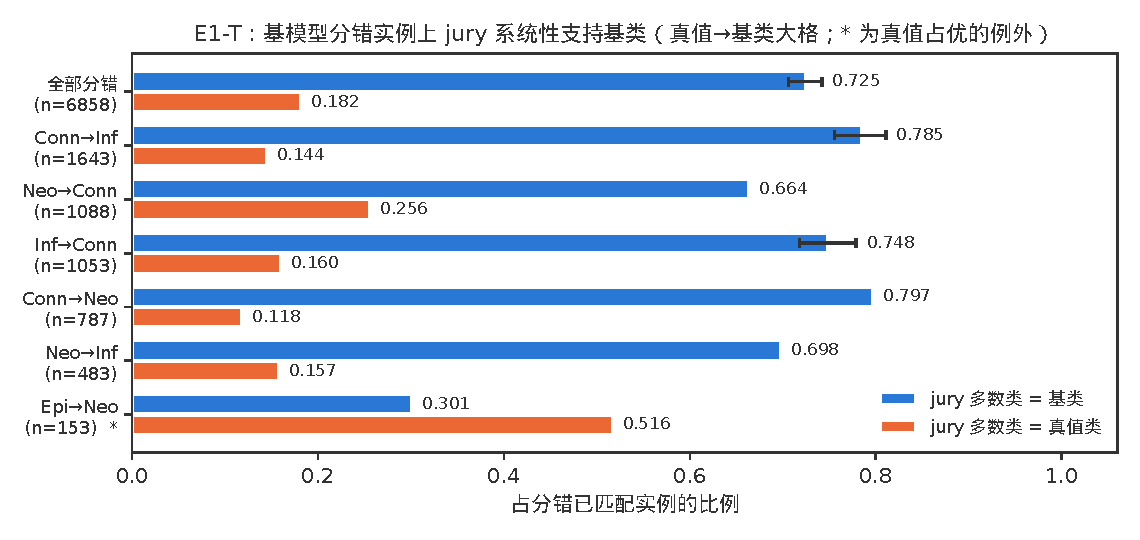
\includegraphics[width=\linewidth]{figs/e1t_pairs_zh.pdf}
\caption{E1-T 主要（真值$\to$基类）混淆组中评审团多数类的归属。前三行带 bootstrap 区间（横线）。Epi$\to$Neo（星标）是唯一以真值类别占优的主要混淆组。}
\label{fig:e1t}
\end{figure}

G1 内评审团多数类与基类一致的比例是 72.5\%，与真值类一致只有 18.2\%，两个置信区间不重叠；作为对照，基模型分对的实例上，评审团的改判率仅 1.9\%。G0 的作用在于约束“完全复制基模型输出”的解释：如果评审团只是复制基模型的输出，G0 改判率应接近零且 G1 应接近 100\%，观测结果均不符合完全复制的情况，但仍不能排除共享偏差。

按（真值$\to$基类）分解，Inf/Conn 双向是样本最多的两组混淆：GT=Inf、基=Conn 的 1,053 例中 74.8\% [0.718, 0.779] 支持基类；GT=Conn、基=Inf 的 1,643 例中 78.5\% [0.756, 0.811]。Neoplastic 指向 Inf/Conn 的两组主要混淆（69.8\%/66.4\%）同向。唯一的例外是 GT=Epi、基=Neo（153 例）：真值占优（51.6\% 对 30.1\%），单列不并入结论。Dead 相关混淆组合计 404 例，多数类 $=$ 基类的区间为 [0.573, 0.703]、$=$ 真值类 [0.173, 0.282]，方向与 Inf/Conn 相同但幅度低、各组结果不一致，按预注册只作描述。

三套敏感性检验同向：配对门槛提高到 IoU 0.5 时 72.0\%；总票门槛提高到 5 时 72.3\%；只用两席 HoVer-Net 组成子评审团时，基类 36.0\% 仍高于真值类 20.2\%（无多数 36.2\%，G0 改判 6.7\%）——跨架构子集上差异减小，但方向一致。

\subsection{结论与边界}

按预注册判读规则，\textbf{结果支持 Inf/Conn 标签边界模糊这一解释，证据来自检测器分类结果的一致性}。T0--T3 与此前 CONCH 实验均未改善分型，E1-T 则发现，多个检测器经常对同一实例给出与基模型一致、却与标注不同的类别。这提示分型缺口可能部分来自标签边界不清，但也可能反映模型共享的偏差。现有证据不能确定两者各占多少，也不能据此断定联合训练无效；本阶段不启动联合训练。

边界必须写清楚。这是检测器一致性证据，不是生物学断言：评审团成员与基模型共享 CellViT 配方（10/12 席），其泛化模式与基模型相关；HoVer-Net 子评审团提供了唯一的跨架构对照，差异减小，但方向一致。单一划分（split 1 验证折）、单一基模型；“标签模糊”是对统计模式的解释，不是对 PanNuke 标注流程的指控。它与 E1-C 的检出结果的一致性一起，构成类别判断与核是否存在这一问题两条标签质量证据链，但两类证据都止步于“标签可疑”，不量化噪声率。

\section{E3：候选质量学习的开发轮}

\subsection{设计与五组方案的离线比较}

E1-C 显示支持度单调预测候选的真值匹配。E3\cite{specs}据此检验更强的命题：学习到的质量分数能否替代手工 EF 规则。训练数据是 fold 1 的 13,332 条折外候选（split 2 三种子生成，fold 1 是其验证折，折外成立），标签为冻结的 matched 列；应用侧是 split1\_seed1 的 4,084 个冻结候选，在 fold 2 上比较五组方案：A0 identity、A1 冻结 EF-P2（原有方案，a30d）、A2 纯面积区间、A3 低维特征学习质量（12 维：面积、延展率、圆度、距离、置信度、边缘余量、触边标记、类别 one-hot）、A4 加评审团支持度。模型为逻辑回归，超参由 fold 1 内部分组交叉验证选择。fold 3 零读取；fold 2 的匹配标签只允许出现在端点评测。

每组内部的选择规则逐字沿用 EF 轮：在 mPQ、bPQ $\geq$ identity$-0.002$，strict Dead $\geq$ identity，内部 Dead 匹配数超过 identity 的候选行中，取验证 mPQ 最高者。A1 重放对冻结 EF-P2 选择结果进行严格一致性检查（差值 $\leq10^{-12}$），其中 a30 变体曾逐位复现 EF 轮的 mPQ 0.48346，由此确认重放流程与原流程一致。

主要判定条件要求相对 A1：$\Delta$Dead $\geq+0.002$ 且 $\Delta$bPQ $\geq-0.0005$ 且 $\Delta$strict Dead $\geq-0.002$；次要判定条件要求同等 Dead 增益下误报添加至少减少 25\%。任一条件通过则进入确认轮；两项条件均未通过则结束实验，不扩展候选配置，也不更换模型。

\subsection{结果：三组方案均未通过两项判定条件}

\begin{table}[H]
\centering\small
\caption{E3 关键行的 fold 2 端点。候选配置取 A2--A4 候选配置集中 strict Dead 最高者与按官方指标表现较好的配置两行；相对差值为各组所选配置相对 A1 之差。}
\label{tab:e3}
\begin{tabular}{lrrrrrr}\toprule
行 & mPQ & bPQ & Dead PQ & strict Dead & 添加数 & 未匹配占比\\\midrule
A0 identity & 0.48221 & 0.65093 & 0.16104 & 0.12957 & 0 & —\\
A1 冻结 EF-P2 & 0.48346 & 0.65218 & 0.16714 & 0.13448 & 1,374 & 53.3\%\\
a4\_p0.7（候选配置 strict 最高） & 0.48395 & 0.65288 & 0.16547 & 0.12454 & 1,041 & 42.8\%\\
a4\_p0.5（官方指标较优） & 0.48487 & 0.65384 & 0.17011 & 0.12151 & 2,134 & 46.8\%\\
\bottomrule
\end{tabular}
\end{table}

\begin{figure}[H]
\centering
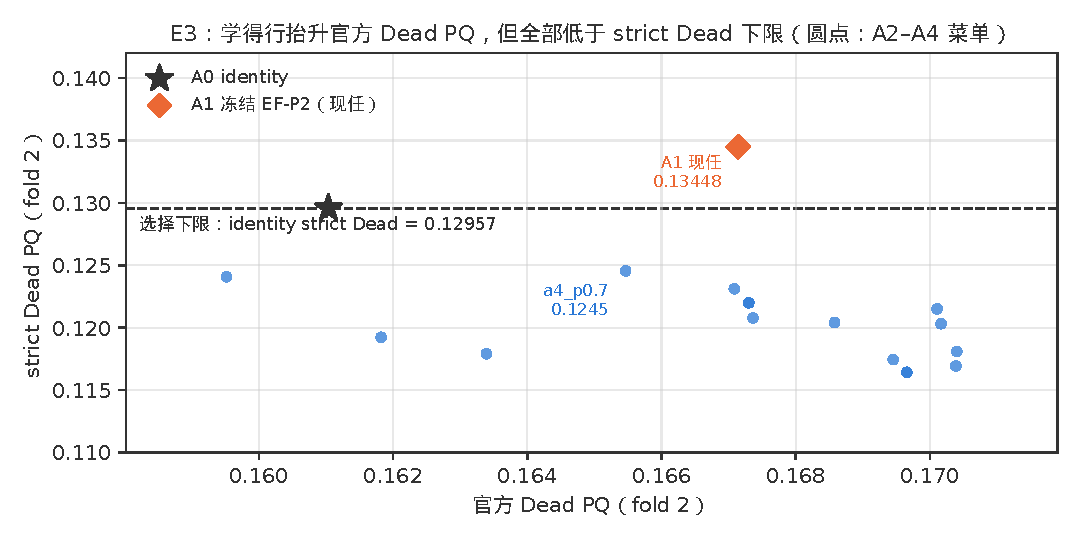
\includegraphics[width=\linewidth]{figs/e3_strict_zh.pdf}
\caption{E3 全部候选配置（A2--A4 候选配置集）的官方 Dead PQ 与 strict Dead PQ。候选配置确实抬升官方 Dead PQ，但全部位于 identity strict Dead 选择下限之下；通过下限的只有原有方案 A1。}
\label{fig:e3}
\end{figure}

选择规则在 A2、A3、A4 的全部 16 个非恒等配置上均未选出合格方案——原因是未达到 strict Dead 下限，尽管部分配置的官方指标有所改善：候选配置的 strict Dead 最高只到 0.12454，低于 identity 的 0.12957；A1（0.13448）则高于这一下限。三组方案因此全部退回 identity（不添加候选），相对差值即 identity 相对 A1 之差：$\Delta$Dead $-0.0061$、$\Delta$bPQ $-0.0012$、$\Delta$mPQ $-0.0012$（bootstrap 区间全部低于或贴零，mPQ 区间 $[-0.00242,-0.00014]$）。主要判定条件、次要判定条件在三组方案上均为否，按预注册规则停止该方向的实验。

这一结果可从以下几个方面分析：

\begin{enumerate}
\item \textbf{候选匹配概率可以用低成本特征预测。}fold 1 分组交叉验证 AUC：低维 12 特征 0.721，加支持度 0.737；低维特征方案在 fold 2 的可靠性曲线良好（均值 0.45 处实际率 0.49，0.65 处 0.62）。E1-C 的单调性假设在拟合模型上成立，说明这些特征具有一定预测能力。
\item \textbf{候选匹配概率不足以保证严格指标。}冻结的 EF 选择规则会排除导致严格指标下降的候选配置；模型分数排序出的行均未达到规定下限。结果说明“候选级效用”与“严格指标对图像级缺类误报的惩罚”不是一回事。
\item \textbf{官方指标与严格指标给出不同结果。}a4\_p0.5 相对 A1 官方口径全面占优（$\Delta$mPQ $+0.0014$、$\Delta$bPQ $+0.0017$、$\Delta$Dead $+0.0030$，添加 2,134 对 1,374，未匹配占比 46.8\% 对 53.3\%），但代价是 strict Dead $-0.0130$。也就是说，部分配置以较低计算成本改善了官方 Dead/bPQ，但同时增加了缺类图像上的 Dead 误报风险——候选级特征（面积、形状、置信度、支持度）不足以判断“这张图里本来有没有 Dead”。
\item \textbf{加入支持度后出现校准偏差。}加支持度后交叉验证 AUC 提升 $+0.016$，但 fold 1 评审团（6 席 CellViT；HoVer-Net split 2 检查点已在两机磁盘清理中丢失，按 spec 应有的第 7 席缺席，偏差已披露）与 fold 2 评审团（13 席跨折跨架构）构成不同：fold 2 上 0.84 预测概率分组的实际匹配率只有 0.58，校准表现变差，AUC 的提高未转化为最终评测指标的改善。
\end{enumerate}

对照 10 月 9 日的建议稿：E1 支持的“候选质量学习”分支就此结束。简单质量模型（含评审团支持度）不能在官方与 strict 联合口径上替代 EF 规则；若将来重开，需要的是\textbf{图像级缺类风险特征}（如该图的 Dead 先验、组织条件），而不是更复杂的候选级分类器。这一解释仍需另行设计实验检验。EF-P2 的定位（机制证据/教师候选）不变。

\section{过程记录、复核与测试}

本阶段的实现遵循先编写测试、再实现功能的流程，测试与一致性检查发现了多处缺陷，修复后均重新运行。主要问题包括：分型探针的类别索引偏移一位（缓存标签行确定性修复后特征逐位一致）；逐图重建的类型查找表曾用全局编号错连图像（改为逐图构建）；E1-T 的多数类语义从“唯一值”改为像素多数票（真实数据存在 164 个未类型化实例）；E1-T 条件 bootstrap 两处口径缺陷（组外行计 0 而非 NaN；先判断事件、再判断是否属于该组）由小规模测试样例暴露；E3 的原有方案绑定曾误用 a30 行——对 a30 的逐位复核确认，原有方案实际为 a30d，改从冻结选择文件确定指标下限并加断言。

实现经独立评审后，E1-T 与 E3 的终版产物重跑再生成，与首版逐位一致（E1-T 全部一致；E3 除 bootstrap mPQ 列外一致，该列口径修正为官方 NaN 排除规则后，identity$-$A1 的 $\Delta$mPQ 区间由 $[-0.00232,-0.00002]$ 改为 $[-0.00242,-0.00014]$，结论不变）；补全了来源记录（EF 选择行、依赖模块指纹、fold 2 真值哈希）。文档与产物的一致性审计 56 项全部通过，其中两处描述数字按产物修正（加入支持度的方案 0.84 预测概率分组实际率 0.58 而非 0.55；支持度 AUC 增益 $+0.016$ 而非 $+0.017$）。此前全量回归测试 \textbf{335 项通过}（本阶段净增 58 项），依赖环境不变。

\section{局限与下一步}

\subsection{本阶段的局限}

\begin{enumerate}
\item \textbf{主要实验仅覆盖单一验证设置。}T、E1-C、E1-M、E1-T、E3 都在 split 1 的验证折上，基模型单一（split1\_seed1）；E3 的训练侧虽覆盖 split 2 三种子，应用侧仍是单一候选池。所有比例的置信区间只反映图像抽样不确定性。
\item \textbf{检测器一致性证据不是生物学结论。}评审团与基模型共享训练配方与架构家族；空对照是合成圆盘；两类标签证据都只能说“标签可疑”，不能量化噪声率，也不能区分漏标、单位差异与共享误报。
\item \textbf{E3 是开发轮判定。}“三组方案均未通过两项判定条件”针对冻结候选配置集与冻结规则；该结果不支持“计算成本较低的候选级特征可替代 EF 规则”，不能据此否定其他质量学习方案。
\item \textbf{上限诊断读了测试产物。}第 2 节访问了历史测试预测（只读、无调参、无新推理），其余实验未读测试折；本阶段没有新增三划分测试成绩，测试折多轮复用的历史限制不变。
\item \textbf{HoVer-Net 席位不完整。}split 2 检查点丢失使 E3 的 fold 1 评审团缺少跨架构席位；E1-C/E1-T 的跨架构证据依赖仅有的两席。
\end{enumerate}

\subsection{下一步}

类别判断与核检出两方面均获得了检测器一致性证据，两条学习线（事后读出、候选效用）都以负结果结束。后续工作建议如下：

\begin{enumerate}
\item \textbf{把标签模糊写进最终报告的分析框架。}Inf/Conn 边界模糊改变了“分型缺口=模型缺陷”的默认解读；组织$\times$类别的误差分解应与检测器一致性证据对照呈现，而不是把缺口全部记为模型损失。
\item \textbf{图像级缺类风险特征。}E3 留下的可检验解释：预测“这张图有没有某类”可能比预测“这个候选是不是核”更有助于控制严格指标所惩罚的缺类误报。若立项，须先写规格（进入条件、对照、停止规则），沿用本轮的预注册纪律。
\item \textbf{联合训练假设保持后置。}它同时改容量、特征与优化日程，只有在标签解释与特征解释都被排除后才值得承担这个成本；当前证据不支持启动。
\item \textbf{人类专家评审仍待完成。}E1 材料包不变；若未来获得两名合格评审，原协议可直接执行，届时检测器一致性证据与生物学判断可以对照。
\end{enumerate}

在上述任何一项立项之前，不启动新的训练，也不在已多轮观察的测试图上扩大筛选规则。

\section{结论}

本阶段针对上一报告提出的两个问题，得到了以下结果。

第一，\textbf{所测试的事后分类方法未改善分型}。真值辅助的类别修正能把 mPQ 从 0.4995 抬到 0.6632，其中约七成与 Inflammatory/Connective 相关；但固定几何的简单读出（聚合、线性头、上下文环）未带来稳定改善，Dead 反而受损。E1-T 随后提供了一种可能解释：基模型分错的实例上，跨折跨架构评审团以 72.5\% [0.706, 0.742] 支持基类、仅 18.2\% 支持真值类，而分对实例上的改判率只有 1.9\%——Inf/Conn 标签边界模糊的检测器一致性证据按预注册判读规则成立。这些结果提示标签边界可能影响分类，但尚不能排除模型共享偏差，也无法证明联合训练不能改善这部分误差。

第二，\textbf{未匹配候选仍需核实，质量模型尚不能替代现有筛选规则}。与真值零重叠的候选中 66--73\% 获得跨折跨架构的多检测器支持（空对照 0.75\%），检测器共同检出这些对象，提示标注可能需要核查；匹配率随支持度单调上升，候选质量模型的交叉验证 AUC 达 0.721/0.737。但沿用冻结选择规则时，此次新增的全部候选配置均未达到 strict Dead 下限，此次候选配置在官方口径上的改善伴随 strict Dead 下降，E3 按预注册规则停止该方向的实验。

复核情况：五项实验中四项纯 CPU 重放、一项含两席验证折推理，未读取测试折、未新增分割模型训练；此前 335 项测试通过，终版产物复核完成（E3 的 bootstrap mPQ 列修正了统计口径），文档-产物审计 56 项通过。本阶段的结果支持在最终报告中纳入标签边界问题，并将图像级缺类风险列为后续待检验方向。

\appendix
\section{文件、数字与复现入口}

\subsection{数值核验}

本报告全部表格数字由 \code{scripts/report5\_numbers.py} 从五份冻结产物导出（快照 \code{runs/analysis/report5\_numbers.txt}）；\code{scripts/verify\_report5.py} 从最底层可用产物独立重算并核对——包括：oracle 当前值与官方基线评测逐位一致、T 通过条件布尔值由存储数值重推、E1-C 支持度直方图与匹配率从 \code{per\_candidate.npz} 加冻结候选记录重算、E1-M 一致率与 kappa 从两轮 CSV 重算、E1-T 分组计数总和等于 fold 2 真值实例数且区间括住点估计、E3 选择规则在全部行上重放并与冻结选择一致——结果写入本目录 \code{verified\_numbers.json}。bootstrap 区间沿用冻结结果，不重新抽样。第 4.2 节的零重叠分层计数由 \code{per\_candidate.npz} 与候选记录的联表重导，因为 \code{consensus.json} 只存聚合值。

图表由 \code{scripts/make\_report\_figures5.py} 从同一批产物生成，数值与 \code{figs/} 内冻结 CSV 一致。

\subsection{产物与复现命令}

\begin{table}[H]
\centering\footnotesize
\caption{主要实验产物，均相对仓库根目录；\code{runs/} 下为本地产物，不随 Git 分发。}
\begin{tabularx}{\linewidth}{lY}\toprule
路径 & 本报告用途\\\midrule
\code{runs/analysis/typing\_oracle\_20261009/} & 分类上限诊断三行表与逐类结果。\\
\code{runs/analysis/typing\_probe\_20261010/} & T0--T3 端点、通过条件与诊断列。\\
\code{runs/analysis/e1\_packet\_20261010/} & E1 盲审材料包（200 窗口，两阶段协议，待评审）。\\
\code{runs/analysis/e1\_consensus\_20261010/} & E1-C 共识、空对照、E1-M 两轮盲评。\\
\code{runs/analysis/e1t\_typing\_20261011/} & E1-T 分组、按混淆组、bootstrap 与敏感性。\\
\code{runs/analysis/e3\_quality\_20261011/} & E3 五组方案端点、选择重放、模型诊断。\\
\code{runs/analysis/report5\_numbers.txt} & 本报告逐表数字快照。\\\bottomrule
\end{tabularx}
\end{table}

在固定依赖环境、仓库根目录执行：
\begin{quote}\small
\texttt{python scripts/report5\_numbers.py}\\
\texttt{python scripts/verify\_report5.py}\\
\texttt{python scripts/make\_report\_figures5.py}\\
\texttt{python -m pytest -q}
\end{quote}
核验脚本在产物缺失或数值不一致时以错误状态退出，不修改实验产物。

\begin{thebibliography}{9}
\raggedright
\bibitem{reports} bdd26 项目. 阶段报告三、四：跨尺度候选筛选与机制对照[R]. 2026-10-06/08. \code{docs/report/stage_report\_3/}; \code{docs/report/stage_report\_4/}.
\bibitem{next} bdd26 项目. 下一步研究计划：先验证能否学到，再决定是否扩展（2026-10-09）[R]. \code{docs/RESEARCH\_NEXT\_2026-10-09.md}.
\bibitem{structure} bdd26 项目. 模型结构、实验复盘与后续方向（2026-10-09 修订）[R]. \code{docs/STRUCTURE\_AND\_STRATEGY\_2026-10-09.md}.
\bibitem{specs} bdd26 项目. 本阶段预注册规格：T 探针、E1 盲审及无专家修订、E1-T 分型共识、E3 候选质量[R]. 2026-10-10/11. \code{docs/superpowers/specs/2026-10-10-typing-probe-t-design.md}; \code{docs/superpowers/specs/2026-10-10-e1-blind-audit-design.md}; \code{docs/superpowers/specs/2026-10-11-e1t-typing-consensus-design.md}; \code{docs/superpowers/specs/2026-10-11-e3-candidate-quality-design.md}.
\bibitem{findings} bdd26 项目. 实验日志：2026-10-09 至 10-12 条目[R]. \code{docs/findings.md}.
\bibitem{pannuke} GAMPER J, ALEMI KOOHBANANI N, BENES K, et al. PanNuke Dataset Extension, Insights and Baselines[EB/OL]. 2020[2026-10-06]. \url{https://arxiv.org/abs/2003.10778}.
\bibitem{cellvit} H\"ORST F, REMPE M, HEINE L, et al. CellViT: Vision Transformers for precise cell segmentation and classification[J]. Medical Image Analysis, 2024, 94: 103143. DOI: \href{https://doi.org/10.1016/j.media.2024.103143}{10.1016/j.media.2024.103143}.
\bibitem{uni} CHEN R J, DING T, LU M Y, et al. Towards a general-purpose foundation model for computational pathology[J]. Nature Medicine, 2024, 30(3): 850--862. DOI: \href{https://doi.org/10.1038/s41591-024-02857-3}{10.1038/s41591-024-02857-3}.
\bibitem{hovernet} GRAHAM S, VU Q D, RAZA S E A, et al. Hover-Net: Simultaneous segmentation and classification of nuclei in multi-tissue histology images[J]. Medical Image Analysis, 2019, 58: 101563. DOI: \href{https://doi.org/10.1016/j.media.2019.101563}{10.1016/j.media.2019.101563}.
\bibitem{kappa} COHEN J. A coefficient of agreement for nominal scales[J]. Educational and Psychological Measurement, 1960, 20(1): 37--46. DOI: \href{https://doi.org/10.1177/001316446002000104}{10.1177/001316446002000104}.
\end{thebibliography}
\end{document}
